\documentclass{tufte-handout}

\usepackage[utf8]{inputenc}
\usepackage[autostyle=true,german=quotes]{csquotes}
\RequirePackage[ngerman=ngerman-x-latest]{hyphsubst}  % für die Trennung von zwei-schrittig
\usepackage[ngerman]{babel}   % neue deutsche Rechtschreibung (z. B. auch für Silbentrennung)

\title{Vorbereitung für das Seminar \enquote{Einführung ins Maschinelle Lernen: Hype oder Hybris}}

\author{Marvin Kastner}

%\date{28 March 2010} % without \date command, current date is supplied

%\geometry{showframe} % display margins for debugging page layout

\usepackage{graphicx} % allow embedded images
  \setkeys{Gin}{width=\linewidth,totalheight=\textheight,keepaspectratio}
  \graphicspath{{graphics/}} % set of paths to search for images
\usepackage{amsmath}  % extended mathematics
\usepackage{booktabs} % book-quality tables
\usepackage{units}    % non-stacked fractions and better unit spacing
\usepackage{multicol} % multiple column layout facilities
\usepackage{lipsum}   % filler text
\usepackage{fancyvrb} % extended verbatim environments
  \fvset{fontsize=\normalsize}% default font size for fancy-verbatim environments

\usepackage{xurl}  % break url

\begin{document}

\maketitle% this prints the handout title, author, and date

\begin{abstract}
\noindent
In diesem Dokument werden die Schritte aufgezählt, die von den Seminarteilnehmern selbständig \emph{vor} Beginn des Seminars auf dem eigenen Laptop durchgeführt werden müssen.
Dies ist notwendig, weil zur Einrichtung der Arbeitsumgebung mehrere Gigabyte Daten heruntergeladen und verarbeitet werden.
Falls Sie während des Seminars keinen eigenen leistungsfähigen Laptop zur Verfügung haben sollten, sprechen Sie bitte frühzeitig die Seminarleitung an.
\end{abstract}

Im Folgenden wird aufgezählt, welche Software und welche Dateien benötigt werden.
Hier gibt es nur manchmal eine zeitliche Abhängigkeit, schauen Sie also gerne schon etwas voraus und parallelisieren Sie Aufgaben da, wo dies den Prozess beschleunigt.


\section{Installation der IDE}

Im Bereich Maschinelles Lernen und Data Science spielen Jupyter Notebooks eine immer größere Rolle%
\cite{perkel_why_2018,hiltch_jupyter_2019}.
Hierbei bezeichnen Jupyter Notebooks gleichzeitig das Medienformat als auch die Standard-IDE.
Diese kann Jupyter Notebooks öffnen, den enthaltenen Code ausführen, die Visualisierungen nah am Code platziert anzeigen und das Ergebnis auch wieder speichern.
Bei der Standard-IDE steht die Seminarleitung bei technischen Problemen umfassend zur Seite.

\begin{marginfigure}
  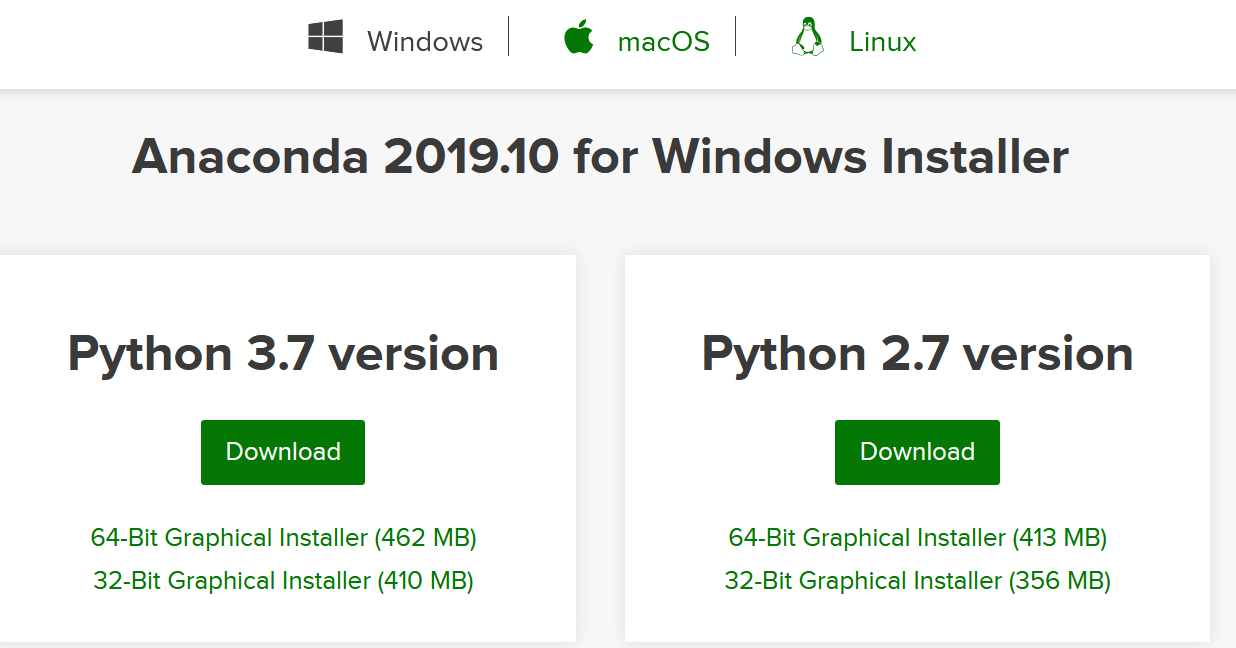
\includegraphics{anaconda}
  \caption{Der Download-Bereich von anaconda.}%
\label{fig:anaconda}
\end{marginfigure}

Anaconda ist eine Python-Distribution, die die IDE \emph{Jupyter Notebook} bereits mit ausliefert.
Unter \url{https://www.anaconda.com/distribution/#download-section} wählen Sie bitte die Version für Python 3 aus.
Dies sollte ungefähr wie in Abbildung\,\ref{fig:anaconda} aussehen.

Falls Sie auf Ihrem PC zwei Accounts, einen Administrator-Account und einen Account fürs alltägliche Arbeiten, verwenden, seien Sie bitte vorsichtig.
Die Installation von Anaconda erfordert keine Administratorenrechte.
Eine Installation mit Administratorenrechten kann u.\,U. dazu führen, dass Anaconda nur für den Administrator installiert ist bzw. dass es zu Problemen mit der Rechteverwaltung kommt.
In der Vergangenheit hat ein erneutes Installieren von Anaconda dieses Problem dann \emph{nicht} beheben können.

Folgen Sie den Installationsschritten und konsultieren Sie im Fehlerfall offizielle Quelle (wie z.\,B. \url{https://docs.anaconda.com/anaconda/install/}) oder Foren.


\section{Bezug der Seminar-Materialien}

Das Seminar besteht aus einer Zusammenstellung von u.\,a. Vorträgen, Diskussionen, gemeinsamem Programmieren und Gruppenarbeit.
Unter \url{https://github.com/1kastner/machine-learning-hype-or-hybris} können Sie die Jupyter Notebooks (diesmal ist das Dateiformat gemeint) herunterladen.
Die Plattform github erlaubt es, dies auf verschiedene Wege zu tun.

\subsection{Klonen mit git}

Für die Versionsverwaltung ist git quasi der Standard und wird immer häufiger auch außerhalb der Software-Entwicklung eingesetzt.
Deswegen lohnt es sich für (fast) jeden, sich Fähigkeiten mit diesem Tool anzueignen.
Das Original-Tool ist ein Kommandozeilentool, welches über \url{https://git-scm.com/} heruntergeladen werden kann.
Wer lieber Visualisierungen mag und klicken können möchte, kann sich eine von vielen GUI Clients%
\sidenote{Eine Liste ist auf \url{https://git-scm.com/download/gui/win} zu finden.}
aussuchen.
Hier sollte natürlich neben dem Betriebssystem auch die Lizenz beachtet werden, falls man den Client später noch mal auf der Arbeit einsetzen möchte.

Installieren Sie sich ein Tool Ihrer Wahl, um dann die aktuelle Version des git-Repositorys \url{https://github.com/1kastner/machine-learning-hype-or-hybris} klonen zu können.
Bis zum Start des Seminars werden u.\,U. die Materialien noch überarbeitet oder erweitert.
Aktualisieren Sie also bitte regelmäßig Ihre vorliegende Version.

\subsection{Download des ZIP-Ordners}

Falls Ihnen git unbekannt ist und Sie keine Zeit dafür haben, sich mit git auseinanderzusetzen, gibt es auch die Möglichkeit, den Inhalt als ZIP-Ordner herunterzuladen.
Klicken Sie dafür auf den Button, wie er in Abbildung\,\ref{fig:github} zu sehen ist.
Falls Lernmaterialien später noch angepasst werden, ist das Zusammenführen der eigenen und der neuen Version allerdings schwieriger.

\begin{marginfigure}
  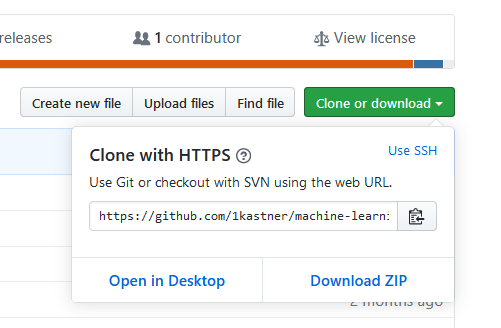
\includegraphics{github-zip}
  \caption{Ein github-Repository bietet verschiedene Möglichkeiten zum Bezug der Inhalte an.}%
\label{fig:github}
\end{marginfigure}




\section{Installation der Bibliotheken}

Die Jupyter Notebooks, die Sie soeben heruntergeladen haben, benötigen jeweils spezielle Bibliotheken.
Einige werden bereits bei der Installation mit Anaconda bereitgestellt, allerdings stehen für das Seminar noch Downloads von weiteren Bibliotheken aus.
Auf der obersten Ebene des git-Repositorys befindet sich die Datei \texttt{environment.yml}, in der alle benötigten Bibliotheken aufgelistet werden.
Diese sollten Sie nun bereits auf dem PC in einem lokalen Ordner Ihrer Wahl vorliegen haben.
Das Format stammt von Anaconda und erlaubt es, die Abhängigkeiten von Bibliotheken automatisch aufzulösen.
Damit man an einem PC in verschiedenen Projekten unterschiedliche Versionen einer gleichen Bibliothek haben kann,
strukturiert Anaconda Bibliotheken standardmäßig in Umgebungen (eng. \emph{environments}.)
Für das Seminar erstellen wir im Folgenden die Umgebung \texttt{ml-hype-or-hybris} basierend auf der gegebenen \texttt{environment.yml}.
Dies kann auf zwei unterschiedlichen Wegen geschehen.

\subsection{conda}

Mit der Installation von Anaconda ist bereits das Kommandozeilentool \texttt{conda} vorhanden.
Unter Windows wird dies je nach Auswahl während der Installation nicht in die Pfad-Variable mit aufgenommen.
Dann steht Ihnen immer noch die \emph{Anaconda Prompt} zur Verfügung.
Weitere Informationen sind auf
\url{https://docs.anaconda.com/anaconda/install/verify-install/#conda}
zu finden.
Eine Übersicht über das Kommandozeilentool ist auf
\url{https://docs.conda.io/projects/conda/en/latest/user-guide/tasks/manage-environments.html#creating-an-environment-from-an-environment-yml-file}
einsehbar.
Dort wird erläutert, wie eine existierende \texttt{environment.yml} eingelesen werden kann.
Folgen Sie der Anleitung und erstellen Sie die passende Umgebung.

\subsection{Anaconda Navigator}

Mit Anaconda Navigator kann die gleiche Aufgabe über eine graphische Oberfläche erledigt werden.
In der Abbildung\,\ref{fig:anaconda-navigator} sehen Sie unten den Button \enquote{Import}.  
Klicken Sie hierauf und behalten Sie den voreingestellten Datentyp \emph{Conda environment file} bei.
Wählen Sie die \texttt{environment.yml} aus und schließen den Vorgang ab.

\begin{figure}[h]
  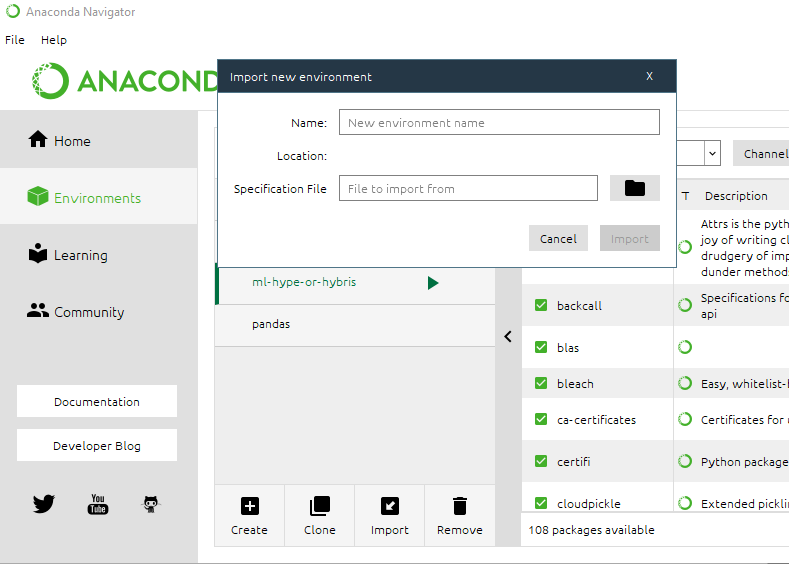
\includegraphics{anaconda-navigator}
  \caption{Der Anaconda Navigator erlaubt das Importieren von \texttt{environment.yml}-Dateien.}%
\label{fig:anaconda-navigator}
\end{figure}




\section{Download von Daten}

Manche der Jupyter Notebooks verwenden Daten, die bereits von den Bibliotheken bereitgestellt werden.
Im Seminar wollen wir aber auch über die Standard-Datensätze hinausgehen.

\subsection{Verkehrsschilder}

Auf \url{http://benchmark.ini.rub.de/index.php?section=gtsrb&subsection=dataset#Downloads} finden Sie den Link zum Download-Archiv.
Laden Sie bitte die Datei \texttt{\detokenize{GTSRB_Final_Training_Images.zip}} herunter und entpacken Sie das ZIP-Archiv.

\bibliography{vorbereitung-auf-das-seminar}
\bibliographystyle{plainnat}

\end{document}
